\documentclass[handout]{beamer}
%Пакеты для математических символов:
\usepackage{amsmath} % американское математическое сообщество.
\usepackage{amssymb} % миллион разных значков и готический, ажурный шрифты.
\usepackage{amscd} % диаграммы, графики.
\usepackage{amsthm} % окружения теорем, определений и тд.
\usepackage{physics} % основные физические символы
%\usepackage{latexsym} % треугольники и пьяная стрелка.

%пакеты для шрифтов:
%\usepackage{euscript} % прописной шрифт с завитушками.
\usepackage{MnSymbol} % Значеки доказательства
\usepackage{verbatim} % улучшенный шрифт "пишущей машинки".
%\usepackage{array} % более удобные таблицы.
%\usepackage{multirow} % мультистолбцы в таблицах.
%\usepackage{longtable} % таблицы на несколько страниц.
%\usepackage{latexsym}

\usepackage{etoolbox}
\usepackage{slashbox} %Разделениени текста \backslashbox{}{}
\usepackage{collectbox} % Добавляет коробочки, можно складывать туда текст)

%Пакеты для оформления:
\RequirePackage[center, medium]{titlesec}% Стиль секций и заголовков
%\usepackage[x11names]{xcolor} % 317 новых цветов для текста.
%\usepackage{multicol} % набор текста в несколько колонн.
\usepackage{graphicx} % расширенные возможности вставки стандартных картинок.
\usepackage{subcaption} % возможность вставлять картинки в строчку
%\usepackage{caption} % возможность подавить нумерацию у caption.
\usepackage{wrapfig} % вставка картинок и таблиц, обтекаемых текстом.
\usepackage{cancel} % значки для сокращения дробей, упрощения, стремления.
%\usepackage{misccorr} % в заголовках появляется точка, но при ссылке на них ее нет.
%\usepackage{indentfirst} % отступ у первой строки раздела
%\usepackage{showkeys} % показывает label формул над их номером.
%\usepackage{fancyhdr} % удобное создание верхних и нижних колонтитулов.
%\usepackage{titlesec} % еще одно создание верхних и нижних колонтитулов

%Пакеты шрифтов, кодировок. НЕ МЕНЯТЬ РАСПОЛОЖЕНИЕ.
\usepackage[utf8]{inputenc} % кодировка символов.
%\usepackage{mathtext} % позволяет использовать русские буквы в формулах. НЕСОВМЕСТИМО С tempora.
\usepackage[T1, T2A]{fontenc} % кодировка шрифта.
\usepackage[english, russian]{babel} % доступные языки.



%Отступы и поля:
%размеры страницы А4 11.7x8.3in
\textwidth=7.3in % ширина текста
\textheight=10in % высота текста
\oddsidemargin=-0.5in % левый отступ(базовый 1дюйм + значение)
\topmargin=-0.5in % отступ сверху до колонтитула(базовый 1дюйм + значение)


%Сокращения
%Скобочки
\newcommand{\inrad}[1]{\left( #1 \right)}
\newcommand{\inner}[1]{\left( #1 \right)}
\newcommand{\infig}[1]{\left{ #1 \right}}
\newcommand{\insqr}[1]{\left[ #1 \right]}
\newcommand{\ave}[1]{\left\langle #1 \right\rangle}


%% Красивые <= и >=
\renewcommand{\geq}{\geqslant}
\renewcommand{\leq}{\leqslant}

%%Значек выполнятся
\newcommand{\per}{\hookrightarrow}


%% Более привычные греческие буквы
\renewcommand{\phi}{\varphi}
\renewcommand{\epsilon}{\varepsilon}
\newcommand{\eps}{\varepsilon}
\newcommand{\com}{\mathbb{C}}
\newcommand{\re}{\mathbb{R}}
\newcommand{\nat}{\mathbb{N}}
\newcommand{\stp}{$\filledmedtriangleleft$}
\newcommand{\enp}{$\filledmedsquare$}

\makeatletter
\newcommand{\sqbox}{%
    \collectbox{%
        \@tempdima=\dimexpr\width-\totalheight\relax
        \ifdim\@tempdima<\z@
            \fbox{\hbox{\hspace{-.5\@tempdima}\BOXCONTENT\hspace{-.5\@tempdima}}}%
        \else
            \ht\collectedbox=\dimexpr\ht\collectedbox+.5\@tempdima\relax
            \dp\collectedbox=\dimexpr\dp\collectedbox+.5\@tempdima\relax
            \fbox{\BOXCONTENT}%
        \fi
    }%
}
\makeatother
\newcommand{\mergelines}[2]{
\begin{tabular}{llp{.5\textwidth}}
#1 \\ #2
\end{tabular}
}
\newcommand\tab[1][0.51cm]{\hspace*{#1}}
\newcommand\difh[2]{\frac{\partial #1}{\partial #2}}


\usetheme{Madrid} % Выбор темы
\usecolortheme{default} % Выбор цветовой схемы
\title{Самодифракция и самофокусировка}
\author{Карибджанов Матвей}

\begin{document}



\begin{frame}% первый слайд
    \titlepage
\end{frame}

\begin{frame}
    \frametitle{Основа нелинейной теории}
    \begin{columns}
        \begin{column}{0.5\textwidth}
            \begin{equation*}
                P = f\inner{E} \approx \kappa_1 E + \kappa_2 E^2 + \kappa_3 E^3 + o(E^4)
            \end{equation*}

            \begin{column}{0.35\textwidth}
                $E < \cfrac{e}{a^2}$

                $P \approx \kappa_1 E$
            \end{column}
            \begin{column}{0.65\textwidth}
                $E > \cfrac{e}{a^2}$

                $P \approx \kappa_1 E + \kappa_2 E^2 + \kappa_3 E^3$
            \end{column}

            \begin{eqnarray*}
                P & = & \cfrac{\kappa_2 E^2}{2} + 
                \inner{\kappa_1 E + \cfrac{3}{4} \kappa_3 E^3} \cos{\omega t} + \\ 
                & + & \cfrac{\kappa_2}{2}E^2\cos 2\omega t + \cfrac{\kappa_3}{4}E^3 \cos 3\omega t  
            \end{eqnarray*}            
        \end{column}

        \begin{column}{0.4\textwidth}
            \begin{figure}[h]
                \centering
                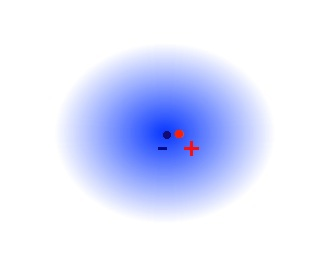
\includegraphics[width=1\textwidth]{polar.jpg}
                \caption{$E_a = \cfrac{e}{a^2} = 10^8 W/cm$}
            \end{figure}
        \end{column}

      \end{columns}
\end{frame}

\begin{frame}
    \frametitle{Самофокусировка}
    \begin{columns}
        \begin{column}{0.5\textwidth}
            \begin{equation*}
                D = E + 4 \pi P = \inner{1 + 4\pi \cfrac{P}{E}} E = \epsilon E
            \end{equation*}

            \begin{eqnarray*}
                n & = & \sqrt{1 + 4\pi \cfrac{P}{E}} = \\
                & = &\sqrt{1 + \cfrac{4 \pi}{E} \inner{\kappa_1 E + \cfrac{3}{4} \kappa_2 E^3}} \approx \\
                & = & \sqrt{1 + \cfrac{4 \pi}{E} \kappa_1} + \cfrac{3/4\kappa_2 E^2}{2\sqrt{1 + \cfrac{4 \pi}{E} \kappa_1}}  \\
                & = &n_0 + n_1 I
            \end{eqnarray*}
        \end{column}
        \begin{column}{0.5\textwidth}
            \begin{figure}[h]
                \centering
                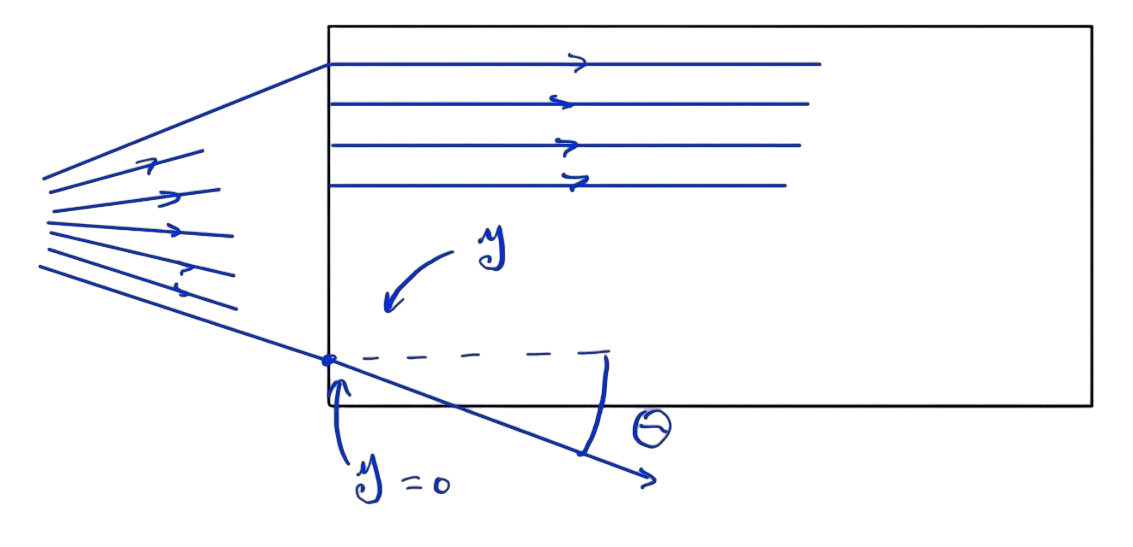
\includegraphics[width=1\textwidth]{self_foc.png}
            \end{figure}
            \begin{equation*}
                \sin \inner{\cfrac{\pi}{2}-\theta} \inner{n_0 + n_2 I}=n_0 
            \end{equation*}
            \begin{equation*}
                \theta^2 = 2\cfrac{n_2}{n_0}I
            \end{equation*}
        \end{column}
    \end{columns}
\end{frame}
\begin{frame}
    \frametitle{Самодифракция}
    \begin{columns}
        \begin{column}{0.5\textwidth}
            \begin{figure}[h]
                \centering
                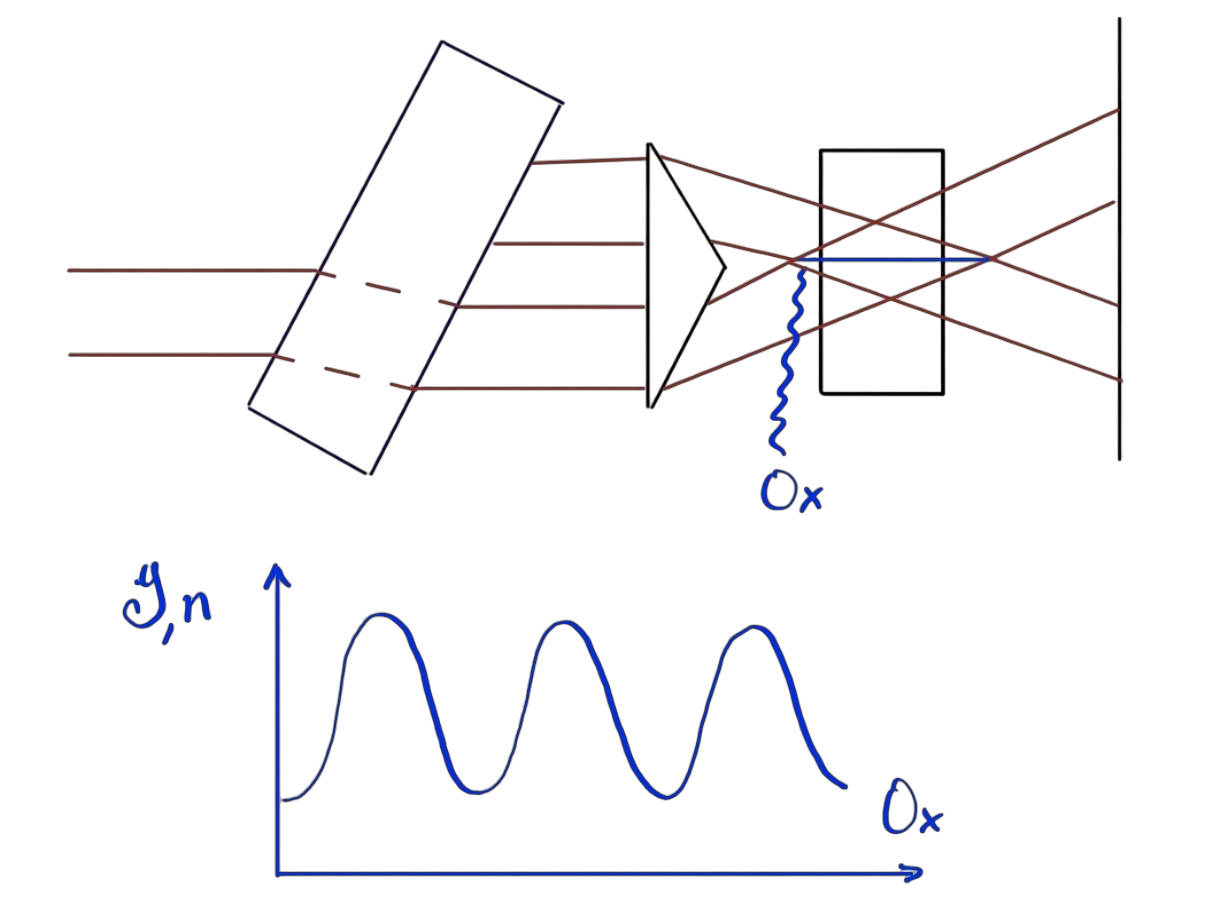
\includegraphics[width=1\textwidth]{self_diff.png}
            \end{figure}

            

        \end{column}
        \begin{column}{0.5\textwidth}
            \begin{equation* }
                I = 2I + 2I\cos \inner{\cfrac{4\pi}{\lambda}n_0 x \sin{2\theta}}
            \end{equation*}

            \begin{equation*}
                n = n_0 + n_2\inner{I} + \Delta n(x)
            \end{equation*}

        \end{column}
    \end{columns}
\end{frame}

\end{document}